\chapter{Implementation}

\section{Git}

Git provides useful information about the current project, the developer is working on, such as:
\begin{itemize}
    \item The current branch (the problem being worked on)
    \item The root directory of the project (for path resolution across devices)
    \item The current version of a file (as a basis for collaborative edits)
    \item Information about the developer (the username)
\end{itemize}

Git stores this information in the ".git" directory in the root folder of the project.
The data is stored in a compressed format. In order to access the information, a small library using low level git commands was implemented. 

It provides functions to:
\begin{itemize}
    \item Find the Git directory for a given file (given the file is inside a git project)
    \item Get the current branch of a Git repository
    \item Get the remote URL for a repository
    \item Get the current version of a given file
    \item Stage a file for commit
    \item Get the username configured for the Git repository
    \item Get a list of branches of a Git repository
    \item Switch a repository to a different branch
\end{itemize}

\section{teletype-crdt}

"The string-wise sequence CRDT powering peer-to-peer collaborative editing in Teletype for Atom."\footnote{https://github.com/atom/teletype-crdt}
This library will be used for tracking changes. It is written in Javascript and currently doesn't include an API documentation.

The main functions used are

\begin{lstlisting}
setTextInRange(start: {row:Number, column:Number}, end: {row:Number, column:Number}, text: string, options?: any): [operation];
\end{lstlisting}
Which is used to notify the document representation about a text operation on the local document and
\begin{lstlisting}
integrateOperations(operations: [operations]): {textUpdates:[textUpdate], markerUpdates:any};
\end{lstlisting}
Which is used to notify the document representation about remote changes and returns the changes to the local file required to keep it in sync with other instances
and
\begin{lstlisting}
undoOrRedoOperations(operationsToUndo: [operation]): any;
\end{lstlisting}
Which is used to undo changes.

\subsection{Git and teletype-crdt}
As a basis for the edit history  the current Git commit in the current branch will be used. teletype-crdt uses numeric siteIds to identify changes. The current Git commit is imported as edited by siteId 1 upon discovering the file.

\section{VS Code Extension API}

VS Code runs extension in a seperate process and provides an asynchronous Javascript API.
The examples provided in the vscode-extension-samples repository\footnote{https://github.com/Microsoft/vscode-extension-samples} are mostly written in Typescript\footnote{https://www.typescriptlang.org/} and all the Interfaces have type definitions for Typescript.
Therefore the Extension will use Typescript as well.

\subsection{Used API functions}

\begin{lstlisting}
vscode.workspace.onDidChangeTextDocument()
\end{lstlisting}

"An event that is emitted when a text document is changed. This usually happens when the contents changes but also when other things like the dirty-state changes."\footnote{https://code.visualstudio.com/api/references/vscode-api\#workspace}

\begin{lstlisting}
vscode.workspace.onDidOpenTextDocument()
\end{lstlisting}

"An event that is emitted when a text document is opened or when the language id of a text document has been changed."\footnote{https://code.visualstudio.com/api/references/vscode-api\#workspace}

\begin{lstlisting}
vscode.workspace.applyEdit(edit)
\end{lstlisting}
"Make changes to one or many resources or create, delete, and rename resources as defined by the given workspace edit."\footnote{https://code.visualstudio.com/api/references/vscode-api\#workspace}

This function returns a promise which resolves when the change has been added to the text document.
An edit is given by a document, the line and column of start and end of the edit in that document and the new text to be inserted there.
If text is added or removed within a line, the columns of the text change after the edit has been applied (when the promise resolves). If another edit is applied before the promise resolved, the indices of the text might have not been changed yet and therefore at a different position than expected. VS Codes WorkspaceEdit supports grouping change operations together. But change operations are not treated as happening all at a time so if for example the text "123" was typed the teletype-crdt library would essentially output Line 1 Char 1 to Line 1 Char 1 changed to "1", Line 1 Char 2 to Line 2 Char 2 changed to "2" and so on. This is kind of expected behaviour so far but VS Code's WorkspaceEdit treats this as independent operations and if there was text after the insertion the changes would not be inserted as 1 block but interlaced with the previous text. 

In order to avoid this race condition all changes to a file have to be carried out sequentially. This is not noticable when changes by regular typing are integrated into the local document. But when the multiple cursors\footnote{https://code.visualstudio.com/docs/getstarted/tips-and-tricks\#\_editing-hacks} are used the change integration can slow down noticably. In order to support multiple cursors the changes are sorted by column in decending order to prevent shifting indices. 
\begin{lstlisting}
textUpdates.sort((a, b) => b.oldStart.column - a.oldStart.column)
\end{lstlisting}

\subsection{Tree View}

In order to stage changes by author, a treeview listing the Authors, who made changes, was created.
The container for a treeview needs to be defined in the package.json file. 

\begin{figure}[]
    \centering
    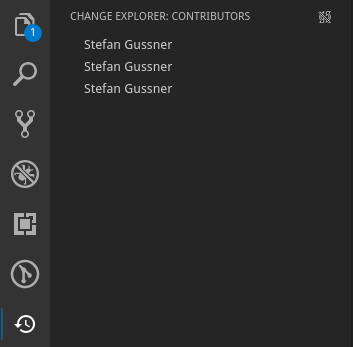
\includegraphics{figures/screenshots/treeview.png}
    \caption{Tree view}
    \label{fig:treeview}
\end{figure}

\begin{lstlisting}[label={lst:contributes_treeview_activitybar}]
"contributes": {
    "viewsContainers": {
        "activitybar": [
            {
                "id": "change-explorer",
                "title": "Change Explorer",
                "icon": "media/icon.svg"
            }
        ]
    }
    [...]
}
\end{lstlisting}

First an entry in the activity bar has to be declared in the viewsContainers section \ref{lst:contributes_treeview_activitybar}. It defines the icon as well as the hover text (called title) of the tab in the activity bar.

\begin{lstlisting}[label={lst:contributes_treeview_view}]
"contributes": {
    [...]
    "views": {
        "change-explorer": [
            {
                "id": "contributors",
                "name": "Contributors"
            }
        ]
    }
}
\end{lstlisting}

Additionally the view has to be declared.\ref{lst:contributes_treeview_view} This defines the heading for the treeview.

\begin{lstlisting}
const treeview = new ContributorsTreeView(crdt.getUsers);
vscode.window.registerTreeDataProvider('contributors', treeview);
\end{lstlisting}